\documentclass{article}%
\usepackage[T1]{fontenc}%
\usepackage[utf8]{inputenc}%
\usepackage{lmodern}%
\usepackage{textcomp}%
\usepackage{lastpage}%
\usepackage{graphicx}%
%
%
%
\begin{document}%
\normalsize%
\section*{December 9, 2017}%
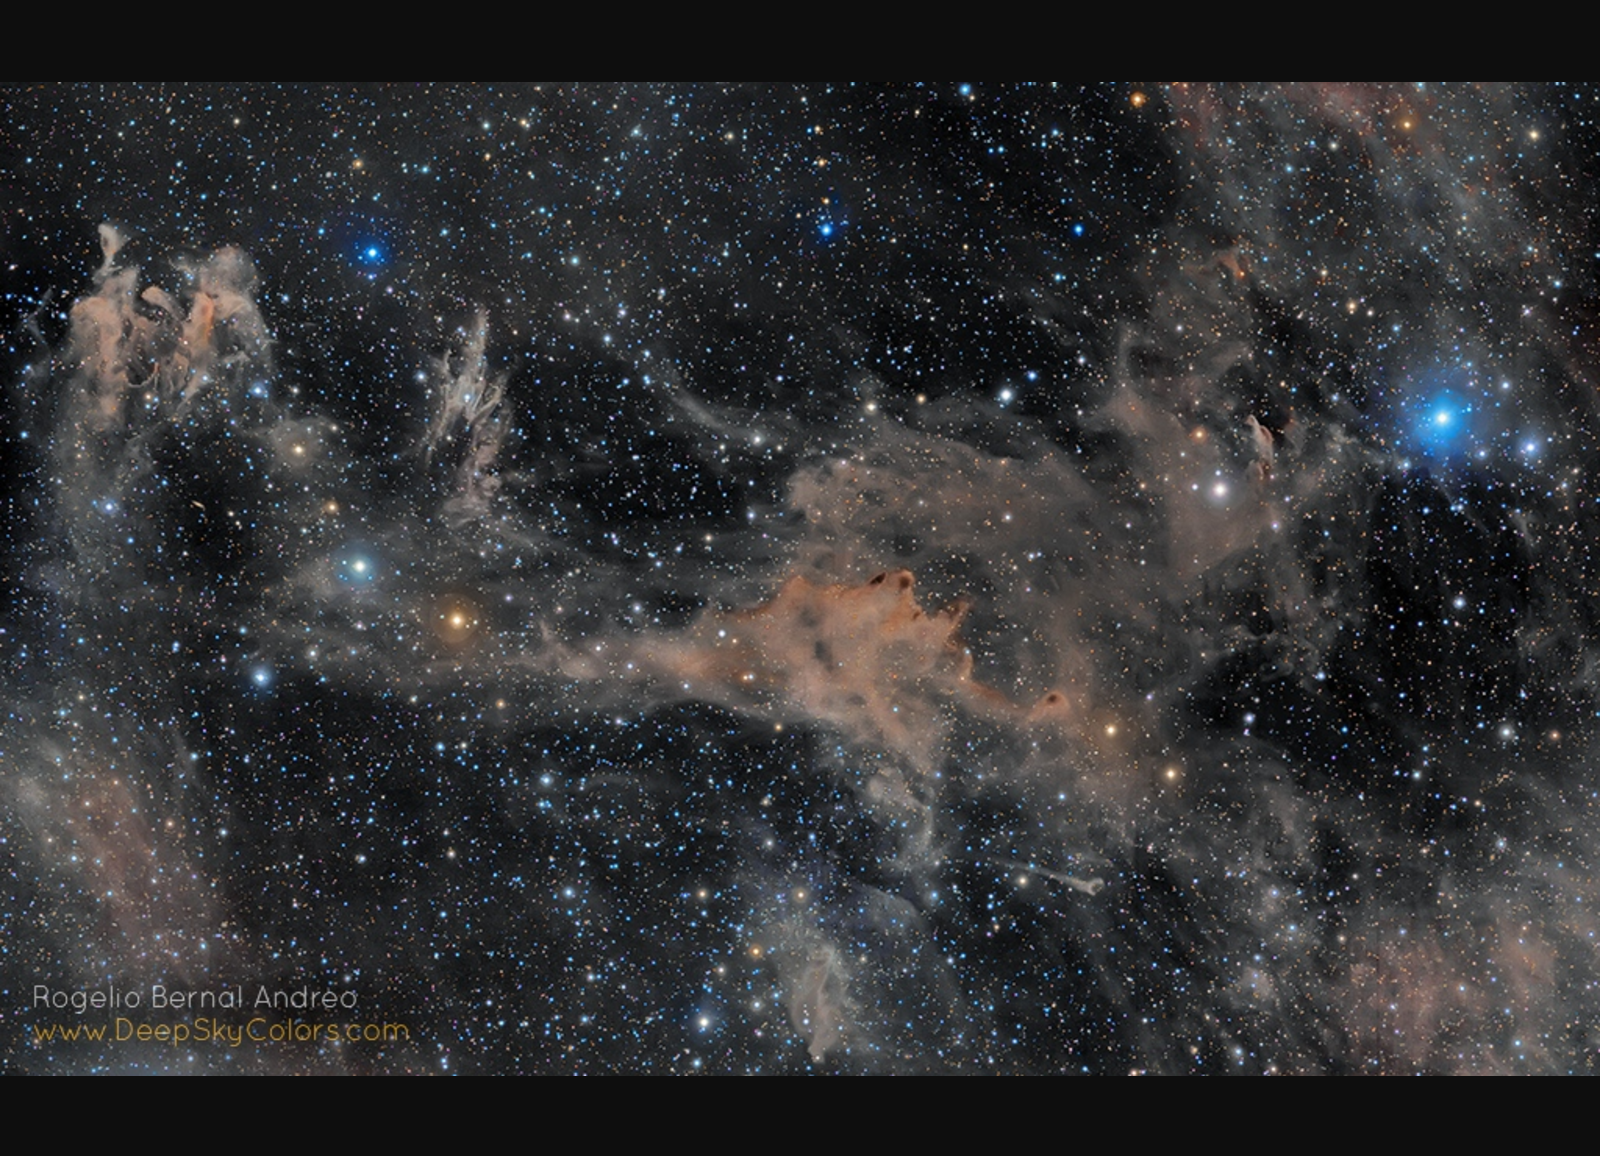
\includegraphics[width=\textwidth]{../lib/pictures/171209.jpg}%
\textbf{\newline%
\newline%
Explanation:\newline%
}%
    This composition in stardust covers over 8 degrees on the northern sky.  The mosaicked field of view is west of the familiar Pleiades star cluster, toward the zodiacal constellation Aries and the plane of our Milky Way Galaxy.  At right in the deep skyscape is bluish Epsilon Arietis, a star visible to the naked{-}eye and about 330 light{-}years away.  Reflecting starlight in the region, dusty nebulae LBN762, LBN753, and LBN743 sprawl left to right across the field, but are likely some 1,000 light{-}years away.  At that estimated distance, the cosmic canvas is over 140 light{-}years across.  Near the edge of a large molecular cloud, their dark interiors can hide newly formed stars and young stellar objects or protostars from prying optical telescopes.  Collapsing due to self{-}gravity, the protostars form around dense cores embedded in the molecular cloud.%
\newpage

%
\section*{December 10, 2017}%
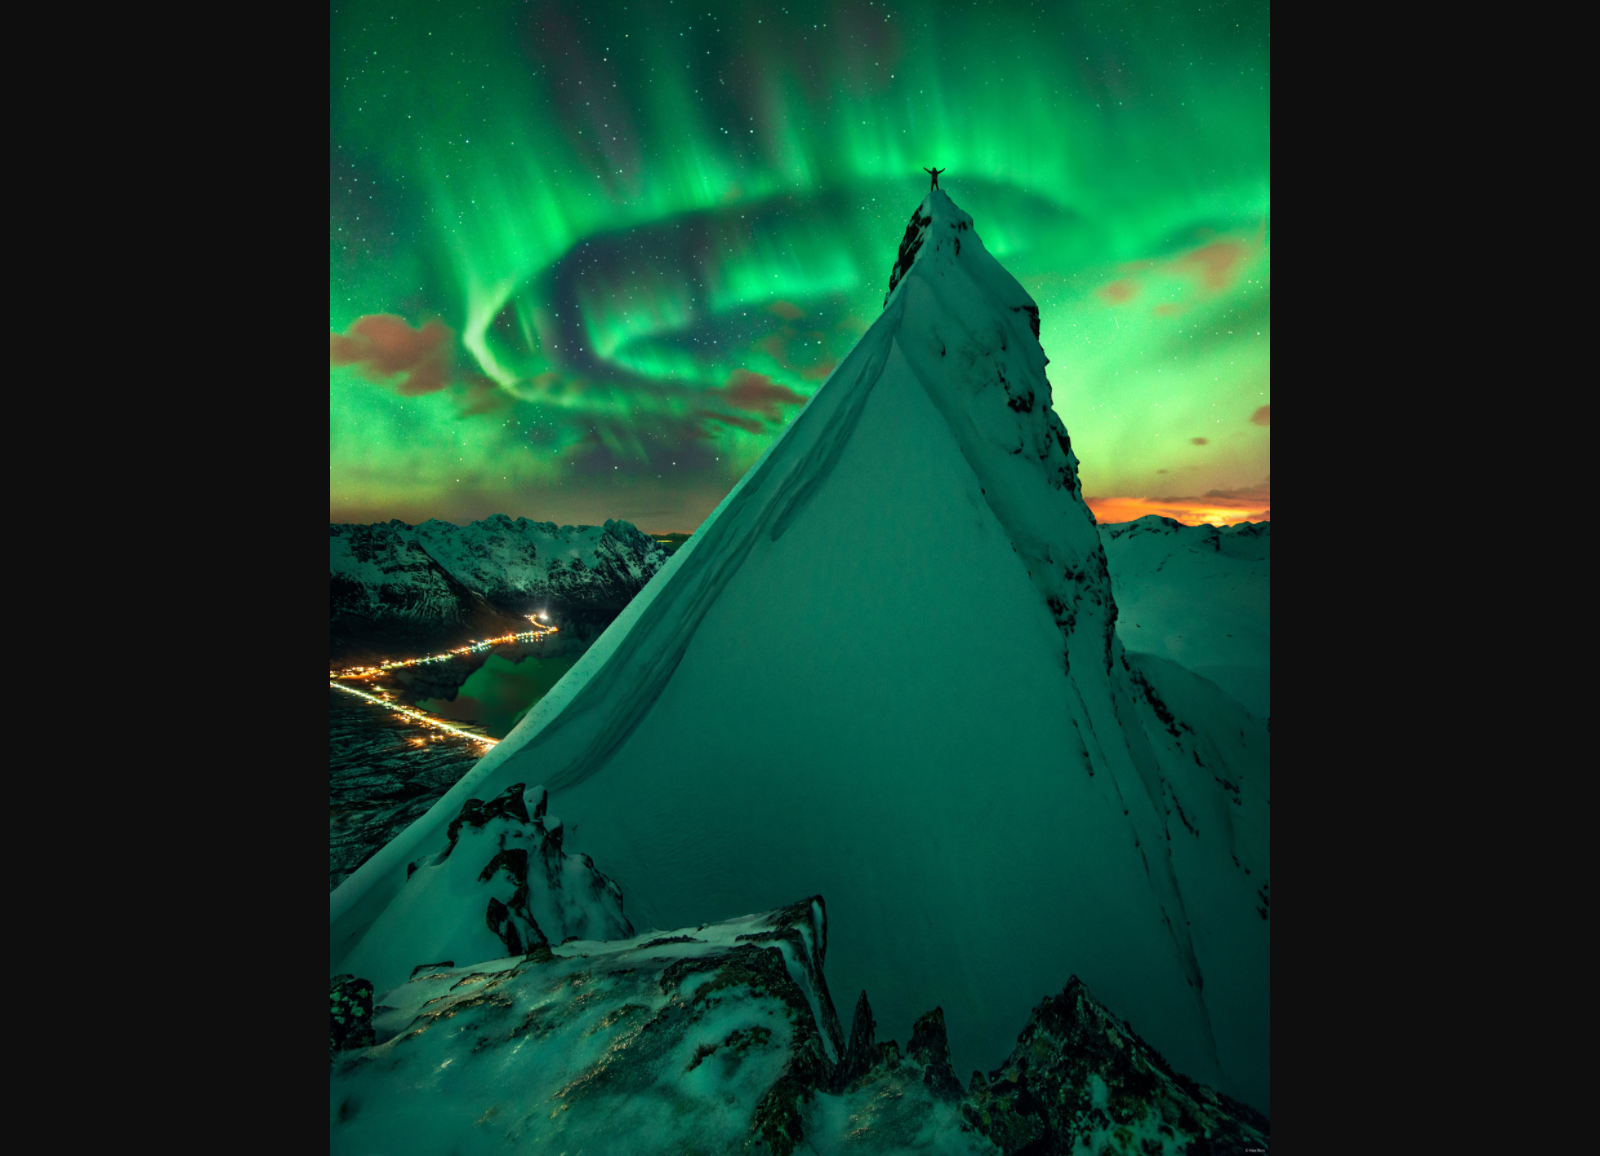
\includegraphics[width=\textwidth]{../lib/pictures/171210.jpg}%
\textbf{\newline%
\newline%
Explanation:\newline%
}%
     Raise your arms if you see an aurora.  With those instructions, two nights went by with, well, clouds {-}{-} mostly.  On the third night of returning to same peaks, though, the sky not only cleared up but lit up with a  spectacular auroral display.  Arms went high in the air, patience and experience paid off,  and the creative featured image was captured as a composite from three separate exposures.  The setting is a summit of the  Austnesfjorden  fjord close to the town of  Svolvear on the  Lofoten islands in northern Norway.  The time was early 2014.  Although our  Sun is nearing  Solar Minimum and hence showing relatively little surface activity,  holes in the upper corona have provided some nice  auroral displays over the last few months.%
\newpage

%
\section*{December 11, 2017}%
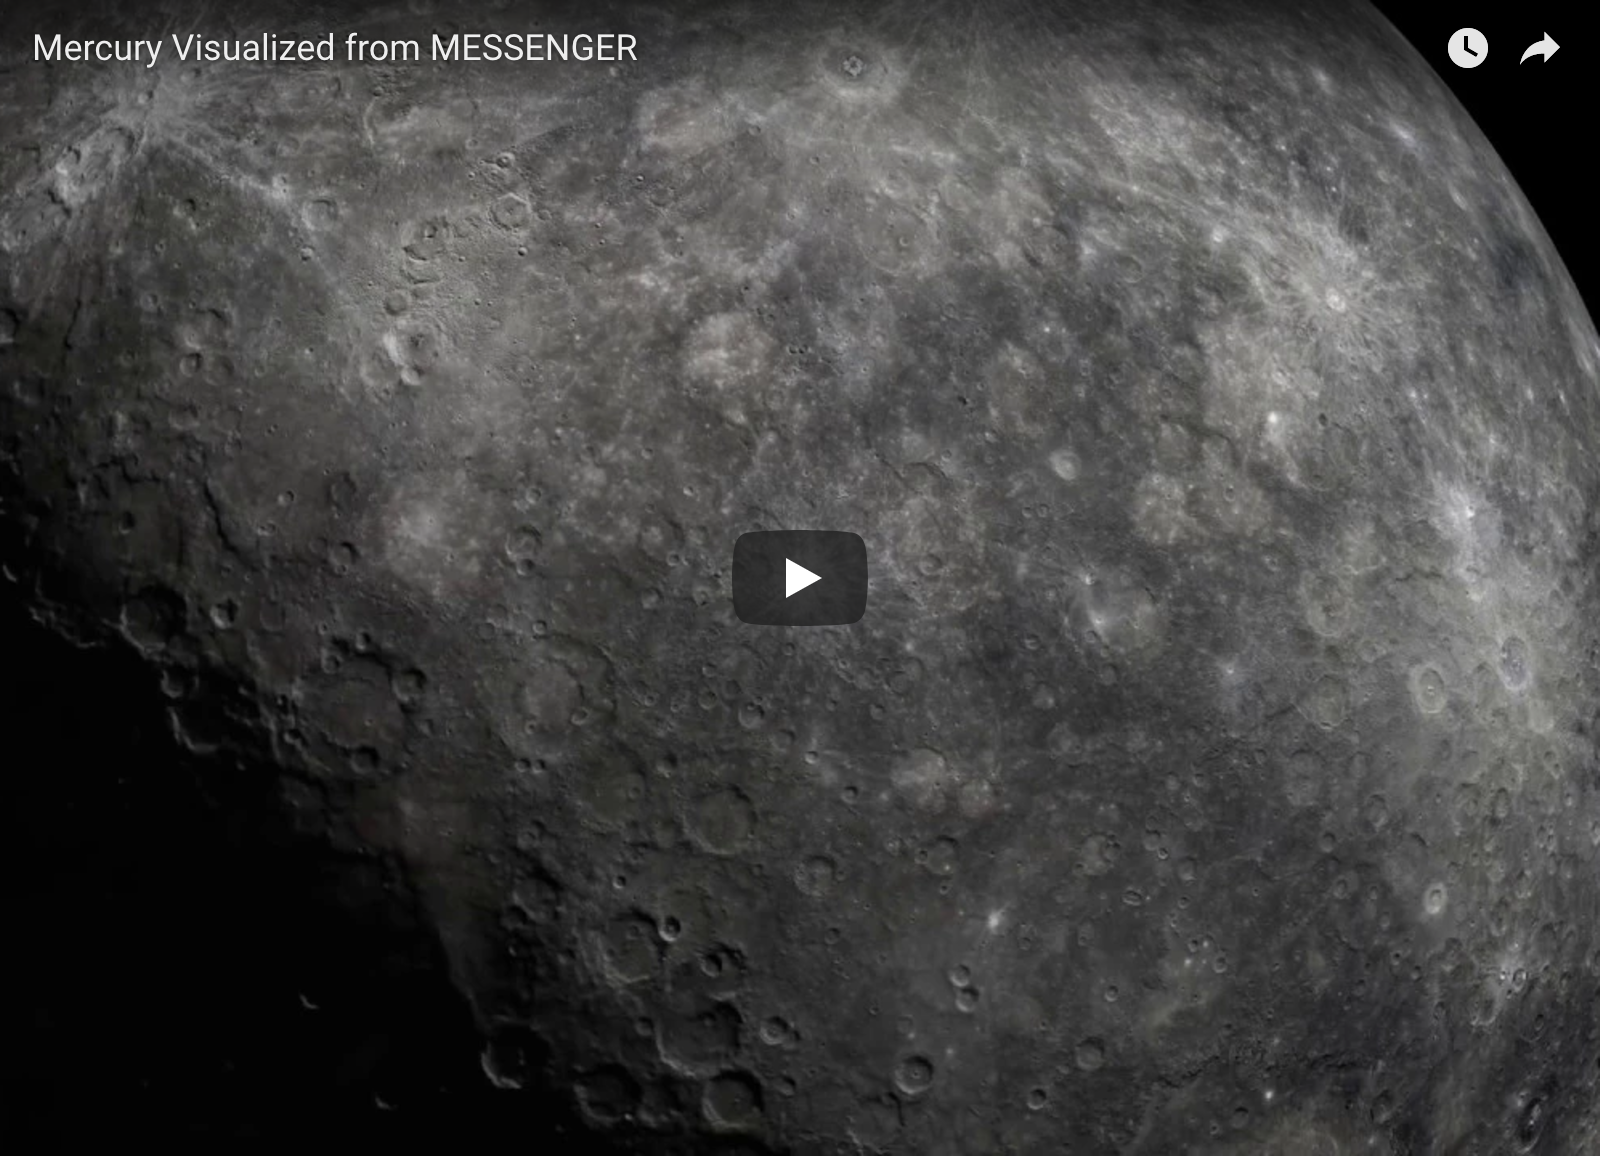
\includegraphics[width=\textwidth]{../lib/pictures/171211.jpg}%
\textbf{\newline%
\newline%
Explanation:\newline%
}%
    What would it be like to fly over the planet Mercury?  Images and data taken from NASA's robotic  MESSENGER spacecraft that  orbited Mercury from 2011 to 2015 have been digitally combined to envision a virtual flight that highlights much of the hot planet's surface.   In general,  the Solar System's innermost world appears similar to  Earth's Moon as it is covered by a heavily cratered gray terrain.  MESSENGER discovered much  about Mercury including that shadows near its poles likely host water ice.   The featured video opens as  Mercury is viewed from the Sun{-}facing side and concludes with the virtual spacecraft  retreating into Mercury's night.   Mercury actually rotates so slowly that it only completes three rotations for every two trips around the Sun.   In 2018, Europe and Japan plan to launch  BepiColombo  to better map Mercury's surface and  probe its  magnetic field.%
\newpage

%
\section*{December 12, 2017}%
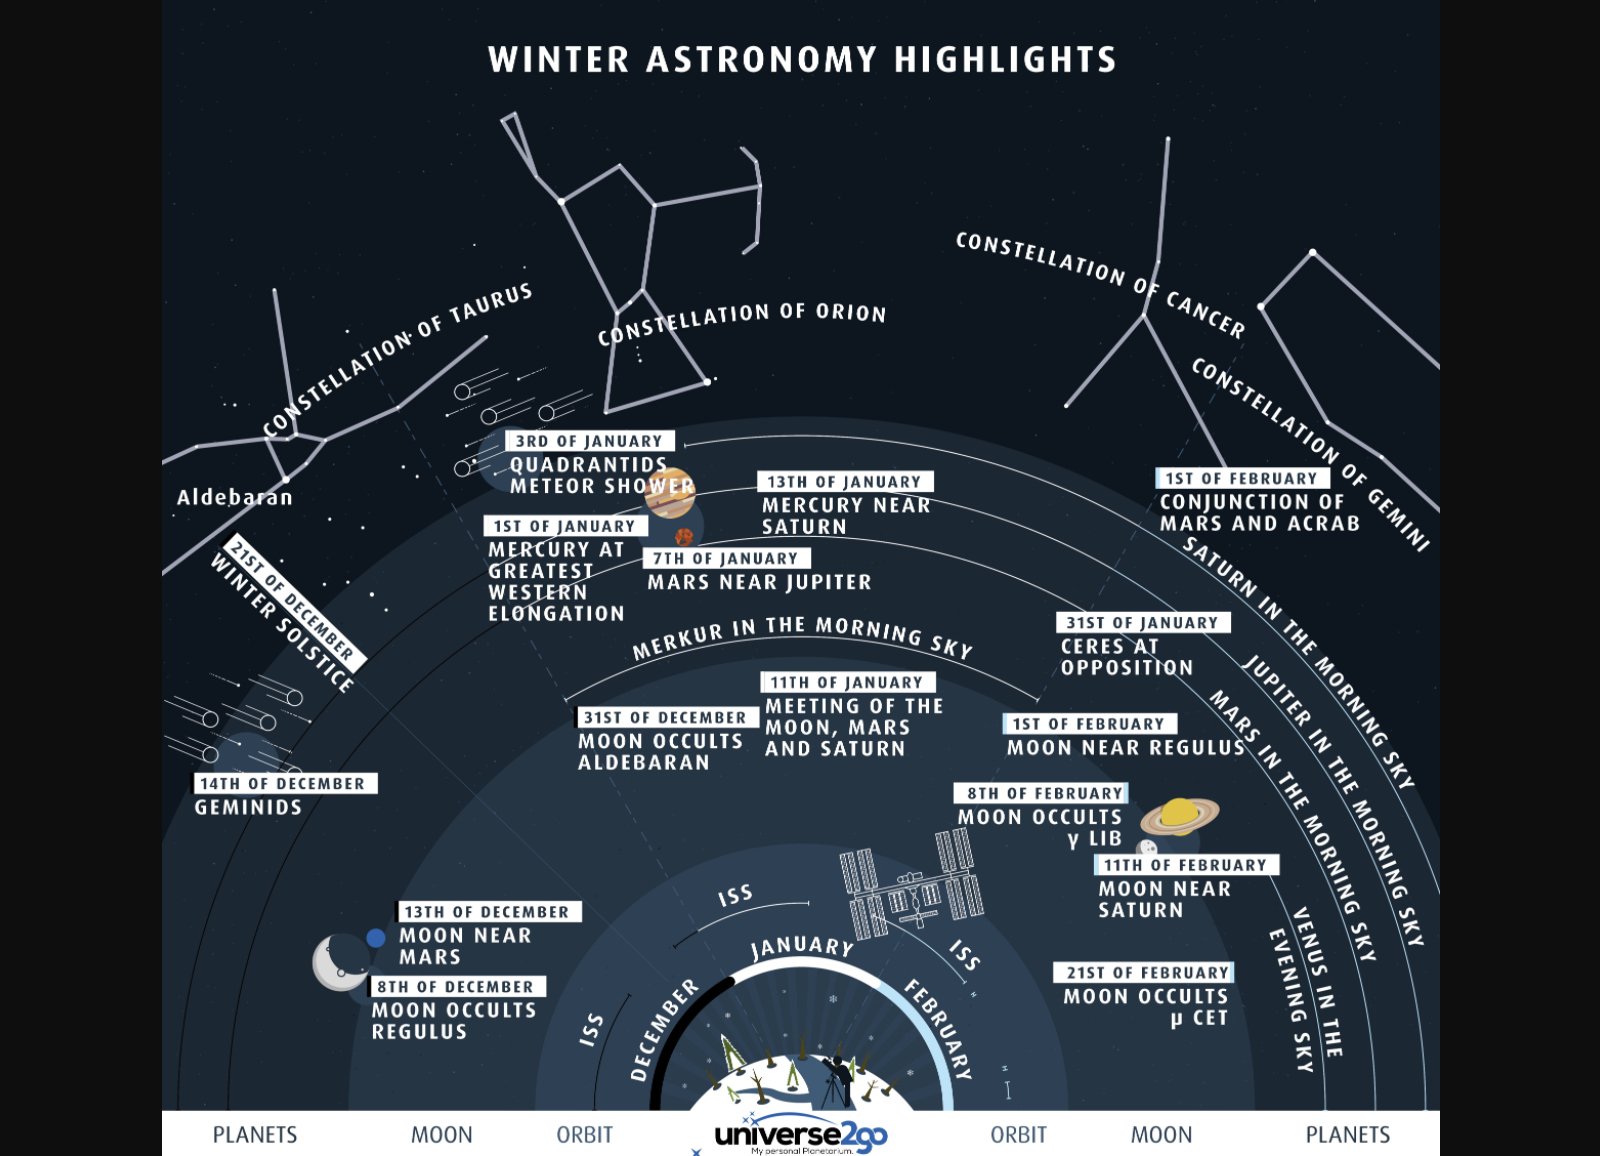
\includegraphics[width=\textwidth]{../lib/pictures/171212.jpg}%
\textbf{\newline%
\newline%
Explanation:\newline%
}%
    What's  up in the sky this winter?   The featured graphic gives a few highlights for Earth's northern hemisphere.   Viewed as a clock face centered at the bottom,  early winter sky events fan out toward the left,  while late winter events are projected toward the right.   Objects relatively close to  Earth are illustrated, in general, as nearer to the cartoon figure with the telescope at the bottom center {-}{-} although almost everything pictured can be  seen without a telescope.   Highlights of this winter's sky include the  Geminids meteor shower peaking this week, the  constellation of Orion becoming notable in the evening sky, and  many planets being visible before sunrise in February.   As true in every season, the  International Space Station  (ISS) can be  sometimes be found  drifting across your sky if you know just when and where to look.%
\newpage

%
\section*{December 13, 2017}%
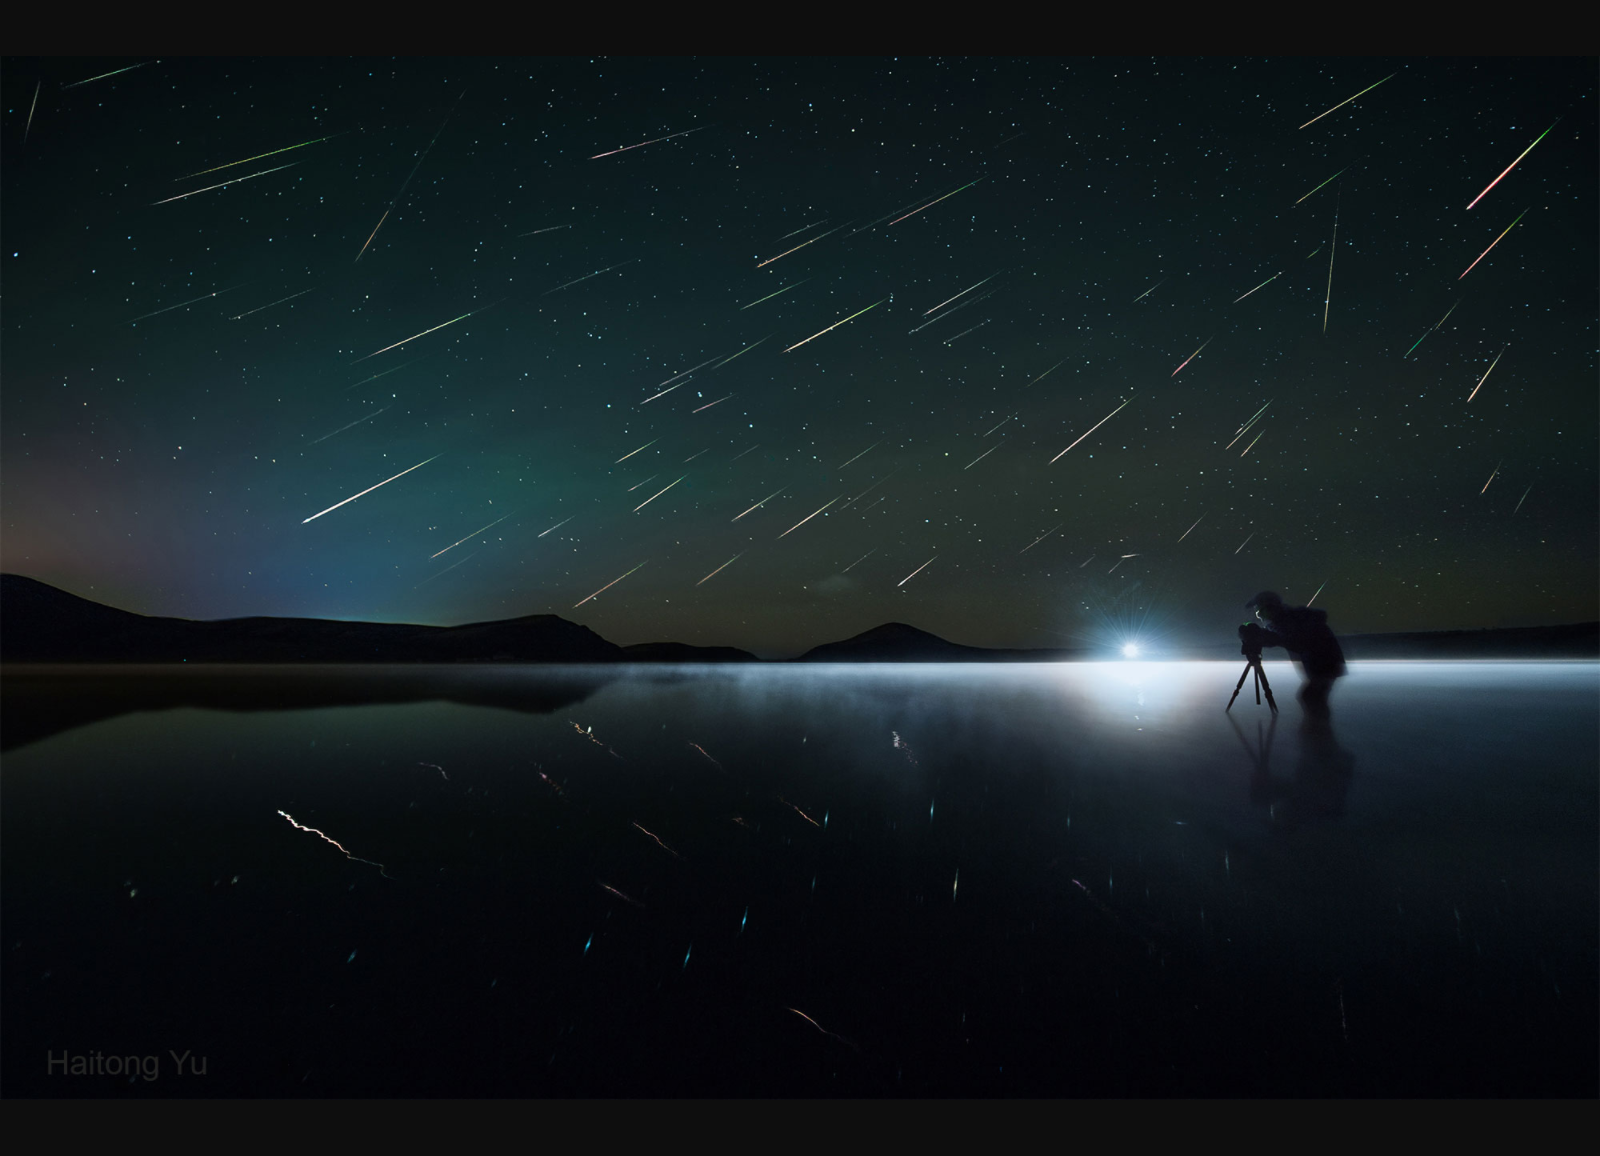
\includegraphics[width=\textwidth]{../lib/pictures/171213.jpg}%
\textbf{\newline%
\newline%
Explanation:\newline%
}%
    Did you ever get caught in a meteor shower?  If yes, then every minute or so the sky sparked with fleeting flashes of light.  This was the fate of the pictured astrophotographer during last year's Perseids  meteor shower.  During the featured three{-}hour image composite,  about 90 Perseids rained down above Lake Duolun of  Inner Mongolia,  China.  If you trace back the meteor streaks, you will find that most of them  appear to radiate from a single constellation {-}{-} in this case  Perseus.  In fact, you can even tell which meteors are not  Perseids because they track differently.  Tonight promises to be another good night to get caught in a meteor shower because it is the peak for the Geminids.  Gemini, the shower radiant,  should rise shortly after sunset and  be visible most of the night.%
\newpage

%
\end{document}